\documentclass{lebook}
\usepackage{lelists}
\setlength{\listtopsep}{0pt}
\setlength{\leftlistindent}{0pt}
\setlength{\rightlistindent}{0pt}

\usepackage{lefonts}
\usepackage{lefontsizes}
\usepackage{lecode}
\codefontsize{\small}

\usepackage{legraphicextensions}
\graphicspath{{Figures/}}

\usepackage{lesubscripts}
\usepackage[pdfauthor={Lance A. Endres}, pdftitle={WinEdt Installation Notes, colorlinks}]{lehyperlink}
\usepackage{leheadersandfooters}

\usepackage{leaddress}

\usepackage{times}

\newcommand{\tbs}{$\backslash$}
\newcommand*{\rootdir}{\textcode{\textit{root}}}
\newcommand*{\supportdir}{\textcode{\textit{support}}}
\newcommand*{\userdir}{\textcode{\textit{user}}}
\newcommand*{\plotstyledir}{\textcode{\textit{plotstyles}}}
\newcommand*{\templatedir}{\textcode{\textit{templates}}}
\newcommand*{\blocksdir}{\textcode{\textit{Blocks}}}

\newcommand*{\rootpath}{\rootdir\tbs}
%\newcommand*{}{}

%%%%%%%%%%%%%%%%%%%%%%%%%%%%%%%%%%%%%%%%%%%%%%%%%%%%%%%%%%%%%%%%%%%%%
% BEGIN DOCUMENT
%%%%%%%%%%%%%%%%%%%%%%%%%%%%%%%%%%%%%%%%%%%%%%%%%%%%%%%%%%%%%%%%%%%%%

\pagestyle{leplainheader}
\begin{document}

\chapter{Installation}
\section{Directories}
\begin{center}
	\begin{tabular}{|l|l|}
		\hline
		% after \\: \hline or \cline{col1-col2} \cline{col3-col4} ...
		\rootdir		& \textcode{C:\tbs{}Custom Program Files\tbs{}CAD Support Files\tbs{}}	\\ \hline
		\supportdir		& \rootpath\textcode{Support}											\\ \hline
		\userdir		& \rootpath\textcode{User Files}										\\ \hline
		\plotstyledir	& \rootpath\textcode{Plot Styles}										\\ \hline
		\templatedir	& \rootpath\textcode{Templates}											\\ \hline
		\templatedir	& \rootpath\textcode{Blocks}											\\ \hline
	\end{tabular}
\end{center}

\section{Command Aliases (PGP)}
\begin{numberedlist}
    \item Open the software's PGP file.
    \item Copy of contents of the \userdir\tbs\textcode{user.pgp} to the bottom of the software's PGP file.  Example file location:
    \begin{plainlist}
    	\item \textcode{C:\tbs{}Users\tbs{}$<$user$>$\tbs{}AppData\tbs{}Roaming\tbs{}ZWSOFT\tbs{}ZWCAD\tbs{}2023\tbs{}en-US\tbs{}Support\tbs{}}
    \end{plainlist}
    \item Close the file and reload it.  The aliases at the bottom will override those at the top.
\end{numberedlist}

\section{Paths}
\begin{numberedlist}
    \item Open the options (command \textcode{options}).
    \item Add the support file path.
    \begin{numberedlist}
    	\item Expand \textcode{File$\rightarrow$Support File Search Path}.
    	\item Add the \supportdir{} directory.
    	\item Move the entry to the top so that anything in that directory is found first.  See \figurename~\ref{fig:addsupportdirectory}.
    	\item Add an entry for each subdirectory in \blocksdir{}.
    \end{numberedlist}
    \item Add the plot style search path.
    \begin{numberedlist}
    	\item Expand \textcode{Printer Support File Path}$\rightarrow$\textcode{Plot Style Table Search Path}
    	\item Add the \plotstyledir{} directory.
    \end{numberedlist}
    \item Add the template files location.
    \begin{numberedlist}
    	% C:\Users\Lance\AppData\Local\Gstarsoft\GstarCAD\R23\en-US\template\
    	\item Expand \textcode{Template Settings}$\rightarrow$\textcode{Drawing Template File Location}
    	\item Add the \templatedir{} directory.
    \end{numberedlist}
\end{numberedlist}

\begin{figure}
	\centering
	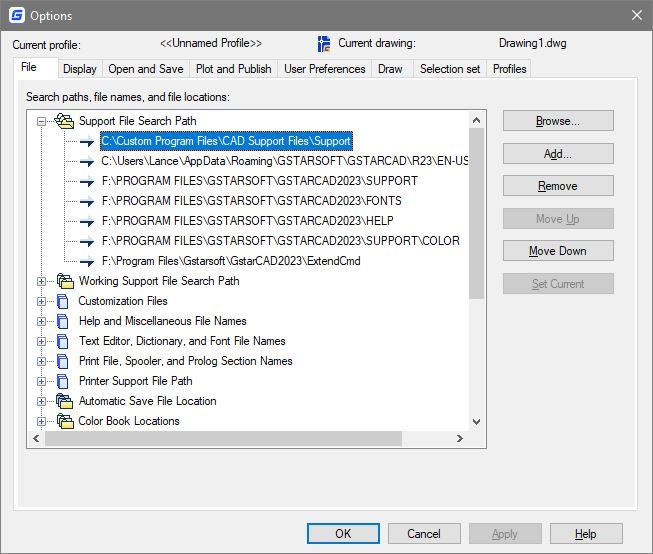
\includegraphics[width=3.25in]{addsupportdirectory}
	\caption{Add the user's support directory to the search path.}
	\label{fig:addsupportdirectory}
\end{figure}


\section{Lisp}
\begin{numberedlist}
    \item Find the software's \textcode{\textit{document}.lsp}.  Examples include:
    \begin{bulletedlist}
    	\item \textcode{acaddoc.lsp}
    	\item \textcode{F:\tbs{}Program Files\tbs{}Gstarsoft\tbs{}GstarCAD2023\tbs{}Support\tbs{}gcad2023doc.lsp}
    	\item \textcode{F:\tbs{}Program Files\tbs{}ZWSOFT\tbs{}ZWCAD 2023\tbs{}Support\tbs{}en-US\tbs{}ZWCAD2023doc.lsp}
    \end{bulletedlist}
    \item Copy it to the \supportdir{} directory.
    \item Edit the file to add the following the end (just before the file \textcode{(princ)} function):
    \begin{plainlist}
    	\item \textcode{; Added to support autoload of custom lisp files.}
		\item \textcode{(load "userdoc.lsp")}
    \end{plainlist}

\end{numberedlist}


\section{Settings}
\begin{bulletedlist}
	\item Turn off \textit{Dynamic Input} (F12) or button at bottom.
	\item Set the crosshair size: \textcode{CURSORSIZE}
	\item Set the right-click customization.
	\begin{numberedlist}
		\item \textcode{OPTIONS}$\rightarrow$\textcode{User Preferences}$\rightarrow$\textcode{Right-click customizations...}
		\item See \figurename~\ref{fig:rightclickcustomization} for the settings.
	\end{numberedlist}
\end{bulletedlist}

\begin{figure}
	\centering
	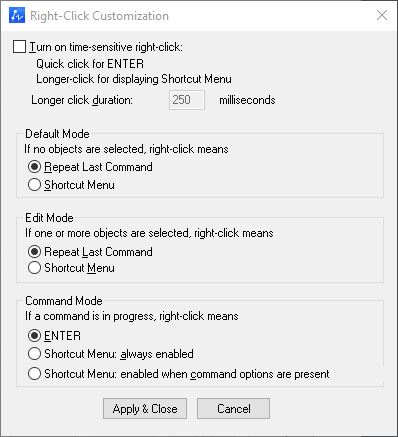
\includegraphics[width=3.25in]{rightclickcustomization}
	\caption{Right-click customization.}
	\label{fig:rightclickcustomization}
\end{figure}


\section{Menus}
\subsection{Load a Partial Menu}
The \textcode{CTRL-D} ortho-toggle is located in the \textcode{lae.mnu} file.
\begin{bulletedlist}
	\item \textcode{MENULOAD}$\rightarrow$lae.mnu (or lae.cuix).
\end{bulletedlist}

\subsection{Set Osnap Menu}
\begin{numberedlist}
	\item Open the \textit{Customize User Interface} (use the command \textcode{CUI}).
	\item Go to \textcode{GCAD/ACAD}$\rightarrow$\textcode{Mouse Buttons}$\rightarrow$\textcode{Shift+Click}$\rightarrow$\textit{Button 2: Snap Button}.
	\item Change \textcode{Macro} from \textcode{\$P0=SNAP \$p0=*} to \textcode{\$P0=lae.SNAP \$p0=*}.
\end{numberedlist}

\subsection{Icons}
The DLL does not seem to load anymore.  Use the \textit{Customize User Interface} to add the icons from the PNG files.

\chapter{Notes}
\section{Using Customizations}
The setup function requires a named plot style drawing to be open.

\section{Programming and Debugging}
\begin{bulletedlist}
	\item \href{https://www.youtube.com/watch?v=Rrgx3TcXNzM}{Video on lisp debugging with GStar2023}
\end{bulletedlist}


\end{document} 